
\subsection{Focus Area - When}
\textbf{Goal:} Understand when contributions from organizations and people are happening
\begin{table}[ht!]
    \centering
    \begin{tabular}{|p{0.35\linewidth} | p{0.6\linewidth}|}
        \hline
        \hfil \textbf{Metric}  & \hfil \textbf{Question} \\
        \hline
		Activity Dates and Times & What are the dates and timestamps of when contributor activities occur? \\ 
		\hline
		Burstiness & How are short timeframes of intense activity, followed by a corresponding return to a typical pattern of activity, observed in a project? \\ 
		\hline
		Review Cycle Duration within a Change Request & What is the duration of a review cycle within a single change request? \\ 
		\hline
		Time to Close & How much time passes between creating and closing an operation such as an issue, change request, or support ticket? \\ 
		\hline
		Time to First Response & How much time passes between when an activity requiring attention is created and the first response? \\ 
		\hline
    \end{tabular}
\end{table}

\hypertarget{activity-dates-and-times}{%
\section{Activity Dates and Times}\label{activity-dates-and-times}}

Question: What are the dates and timestamps of when contributor
activities occur?

\hypertarget{description}{%
\subsection{Description}\label{description}}

Individuals engage in activities in open source projects at various
times of the day. This metric is aimed at determining the dates and
times of when individual activities were completed. The data can be used
to probabilistically estimate where on earth contributions come from in
cases where the time zone is not UTC.

\hypertarget{objectives}{%
\subsection{Objectives}\label{objectives}}

\begin{itemize}
\tightlist
\item
  Improve transparency for employers about when organizational employees
  are engaging with open source projects
\item
  Improve transparency for open source project and community managers as
  to when activity is occurring
\end{itemize}

\hypertarget{implementation}{%
\subsection{Implementation}\label{implementation}}

\hypertarget{filters}{%
\subsubsection{Filters}\label{filters}}

\begin{itemize}
\tightlist
\item
  Individual by Organization
\item
  Aggregation of time by UTC time

  \begin{itemize}
  \tightlist
  \item
    Can show what times across the globe contributions are made; when
    the project is most active.
  \end{itemize}
\item
  Aggregation of time by local time

  \begin{itemize}
  \tightlist
  \item
    Can show what times of day in their local times they contribute.
    Conclusions about the If contributions are more during working
    hours, or if contributions are more during evening hours.
  \end{itemize}
\item
  Repository ID
\item
  Segment of a community, (e.g., GrimoireLab has more EU time zones
  activity and Augur more US time zones activity)
\end{itemize}

\hypertarget{visualizations}{%
\subsubsection{Visualizations}\label{visualizations}}

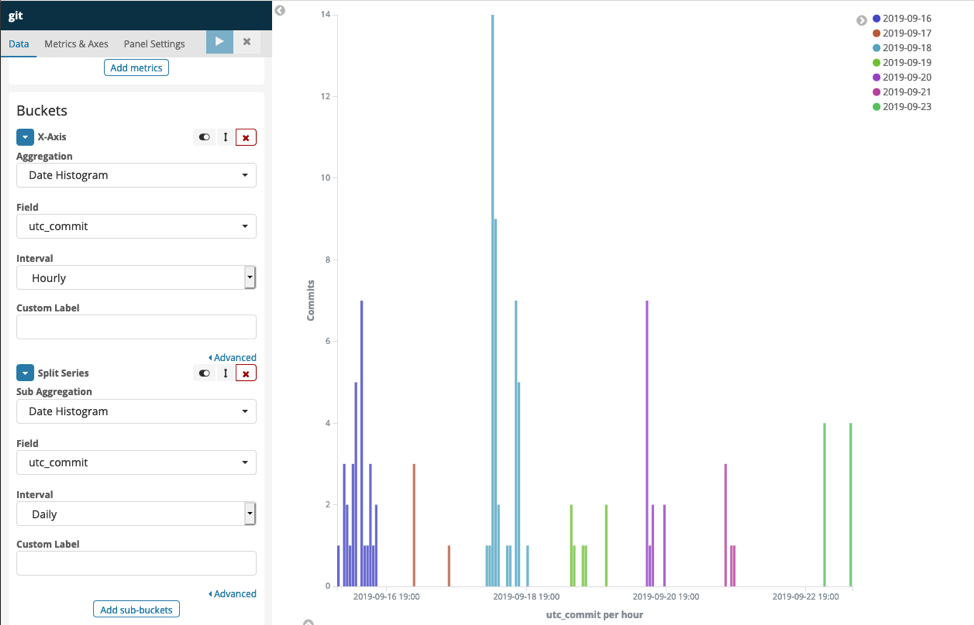
\includegraphics{images/activity-dates-and-times_1.png}
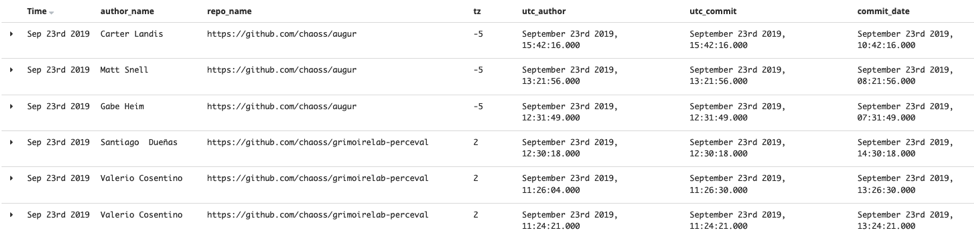
\includegraphics{images/activity-dates-and-times_2.png}
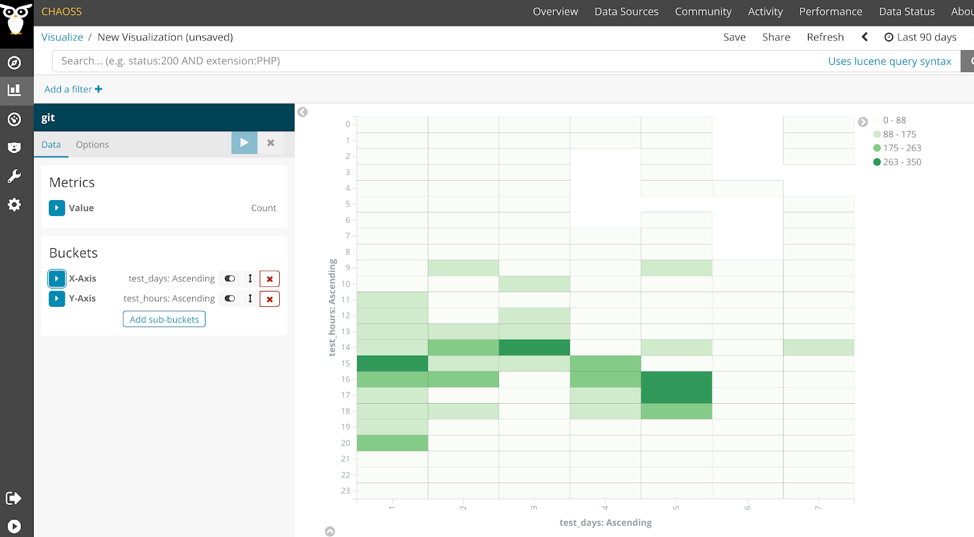
\includegraphics{images/activity-dates-and-times_3.png}
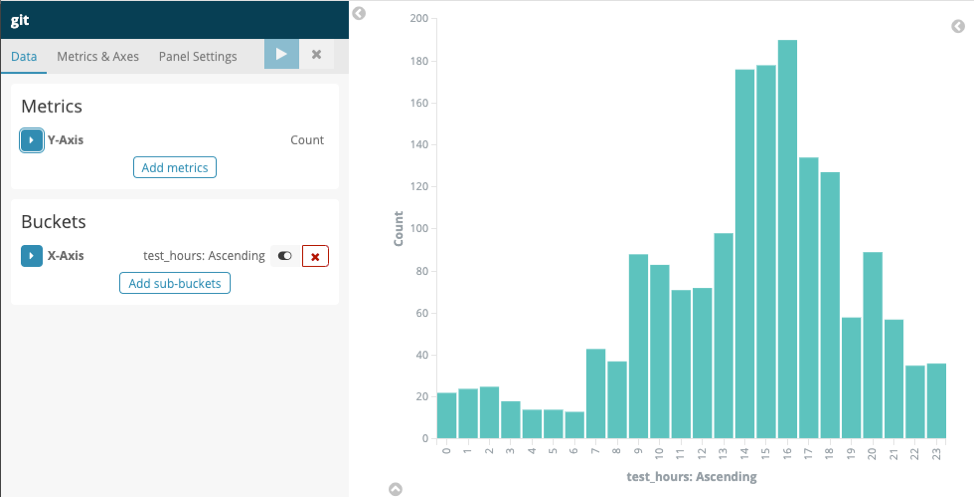
\includegraphics{images/activity-dates-and-times_4.png}

\hypertarget{tools-providing-metric}{%
\subsubsection{Tools Providing Metric}\label{tools-providing-metric}}

\href{https://chaoss.github.io/grimoirelab/}{GrimoireLab}

\href{https://docs.augur.net/\#dates-timestamps}{Augur Date/Timestamps}

\hypertarget{references}{%
\subsection{References}\label{references}}

\href{https://en.wikipedia.org/wiki/Coordinated_Universal_Time}{Coordinated
Universal Time}
 
\hypertarget{burstiness}{%
\section{Burstiness}\label{burstiness}}

Question: How are short timeframes of intense activity, followed by a
corresponding return to a typical pattern of activity, observed in a
project?

\hypertarget{description}{%
\subsection{Description}\label{description}}

There are a number of reasons that may prompt a sudden increase or
decrease in the amount of activity within a repository. These increases
and decreases appear both as a sudden change in activity against the
average amount of activity. Burstiness is a way of understanding the
cycle of activity in existing metrics, like issues, merge requests,
mailing lists, commits, or comments. Examples of root causes for bursts
in activity include:

\begin{itemize}
\tightlist
\item
  Release cycles
\item
  Global pandemics
\item
  Hackathon activities
\item
  Mentorship programs
\item
  Conferences, meetups, and other events where tools are presented
\item
  Conventional and social media announcements and mentions
\item
  Critical bugs as raising awareness and getting people's attention
\item
  Community design meetings or brainstorming meetings to address a
  particular issue
\item
  Community members show up from another community that is relying on
  your project (e.g., dependencies)
\end{itemize}

\hypertarget{objectives}{%
\subsection{Objectives}\label{objectives}}

\begin{itemize}
\tightlist
\item
  To identify impacts of root causes of a burst in activity
\item
  To provide awareness when project activity unknowingly goes up
\item
  To help capture the meaningfulness of increases or decreases in
  project activity
\item
  To help the community and maintainers prepare for future bursts that
  follow a pattern
\item
  To help measure the impact of influential external activities
\item
  To differentiate skewed activity versus normal activity
\end{itemize}

\hypertarget{implementation}{%
\subsection{Implementation}\label{implementation}}

\hypertarget{filters}{%
\subsubsection{Filters}\label{filters}}

\begin{itemize}
\tightlist
\item
  Stars
\item
  Forks
\item
  Issues or bug reports
\item
  Labels
\item
  Downloads
\item
  Release Tags
\item
  Change Requests
\item
  Mail List Traffic
\item
  Documentation additions or revisions
\item
  New Repositories
\item
  Feature Requests
\item
  Messaging Conversations
\item
  Conventional and Social Media Activity
\item
  Conference Attendance and Submissions
\end{itemize}

\hypertarget{visualizations}{%
\subsubsection{Visualizations}\label{visualizations}}

Augur:

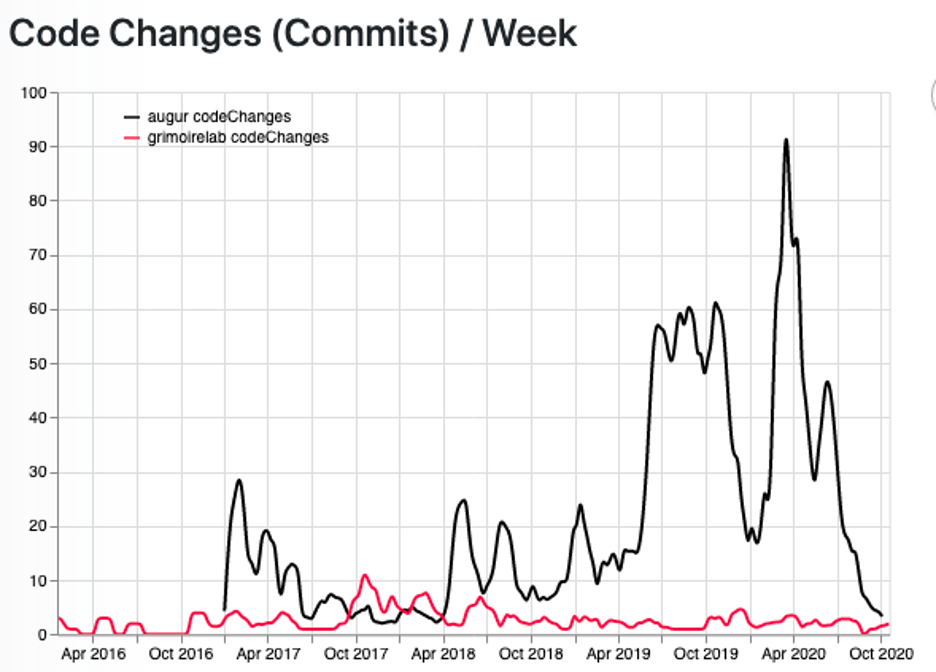
\includegraphics{images/burstiness_augur.png}

GrimoireLab:

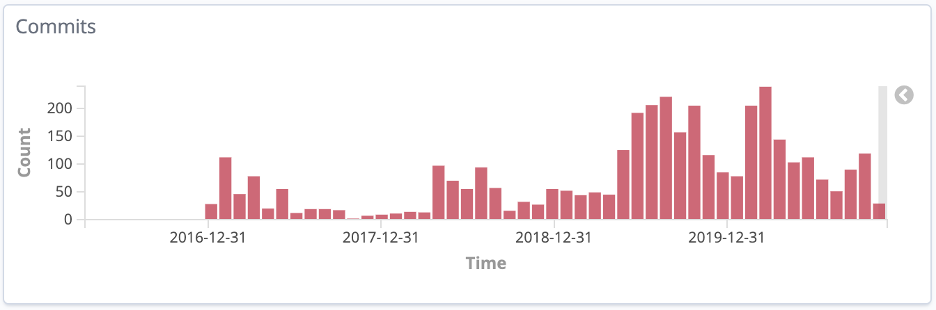
\includegraphics{images/burstiness_gl.png}

\hypertarget{tools-providing-the-metric}{%
\subsubsection{Tools Providing the
Metric}\label{tools-providing-the-metric}}

\begin{itemize}
\tightlist
\item
  Grimoire Lab
\item
  Augur
\end{itemize}

\hypertarget{data-collection-strategies}{%
\subsubsection{Data Collection
Strategies}\label{data-collection-strategies}}

\begin{itemize}
\tightlist
\item
  Quantitative

  \begin{itemize}
  \tightlist
  \item
    Time box activities identifying deviations away from some norm
  \item
    Outliers for certain thresholds, using statistics like Bollinger
    Bands to measure stability or volatility:
    \url{https://en.wikipedia.org/wiki/Bollinger_Bands}
  \end{itemize}
\item
  Qualitative Interview Questions

  \begin{itemize}
  \tightlist
  \item
    Why do you contribute more during a period of time?
  \item
    What do you believe to be the root cause for particular bursts?
  \item
    What impact do different events (e.g., hackathons, mentorship
    program, or conferences) have on project activity?
  \end{itemize}
\end{itemize}

\hypertarget{references}{%
\subsection{References}\label{references}}

This metric was inspired by the work of Goh and Barabasi (2008):
\url{https://arxiv.org/pdf/physics/0610233.pdf}
 
\hypertarget{review-cycle-duration-within-a-change-request}{%
\subsubsection{Review Cycle Duration within a Change
Request}\label{review-cycle-duration-within-a-change-request}}

Question: What is the duration of a review cycle within a single change
request?

\hypertarget{description}{%
\paragraph{Description}\label{description}}

A change request is based on one or more review cycles. Within a review
cycle, one or more reviewers can provide feedback on a proposed
contribution. The duration of a review cycle, or the time between each
new iteration of the contribution, is the basis of this metric.

\hypertarget{objectives}{%
\paragraph{Objectives}\label{objectives}}

This metric provides maintainers with insight on: Code review process
decay, as there are more iterations and review cycle durations increase.
Process bottlenecks resulting in long code review iterations. Abandoned
or semi-abandoned processes in the review cycles, where either the
maintainer or the submitter is slow in responding. Characteristics of
reviews that have different cyclic pattern lengths.

\hypertarget{implementation}{%
\paragraph{Implementation}\label{implementation}}

Review Cycle Duration is measured as the time length of one review cycle
within a single change request. The duration can be calculated between:
The moment when each review cycle begins, defined as the point in time
when a change request is submitted or updated. The moment when each
review cycle ends, either because the change request was updated and
needs a new review or because it was accepted or rejected.

\hypertarget{filter}{%
\subparagraph{Filter}\label{filter}}

Average or Median Duration, optionally filtered or grouped by: Number of
people involved in review Number of comments in review Edits made to a
change request Project or program Organization making the change request
Time the change request was submitted Developers who contributed to a
change request Change request Number of review cycle on a change request
(e.g., filter by first, second, \ldots{} round)

\hypertarget{visualizations}{%
\subparagraph{Visualizations}\label{visualizations}}

\hypertarget{tools-providing-the-metric}{%
\subparagraph{Tools Providing the
Metric}\label{tools-providing-the-metric}}

\hypertarget{references}{%
\paragraph{References}\label{references}}

Example of data that could be used to develop the metric:
\url{https://gerrit.wikimedia.org/r/c/mediawiki/core/+/194071}
 
\hypertarget{time-to-close}{%
\section{Time to Close}\label{time-to-close}}

Question: How much time passes between creating and closing an operation
such as an issue, change request, or support ticket?

\hypertarget{description}{%
\subsection{Description}\label{description}}

The time to close is the total amount of time that passes between the
creation and closing of an operation such as an issue, change request,
or support ticket. The operation needs to have an open and closed state,
as is often the case in code review processes, question and answer
forums, and ticketing systems.

Related metric:
\href{https://chaoss.community/metric-issue-resolution-duration/}{Issue
Resolution Duration}

\hypertarget{objectives}{%
\subsection{Objectives}\label{objectives}}

\begin{enumerate}
\tightlist
\item
  Determining how responsive a community is can help efforts to be
  inclusive, attract, and retain new and existing contributors.\\
\item
  Identifying characteristics of operations that impact an operation
  closing quickly or slowly (e.g., finding best practices, areas of
  improvement, assess efficiency).\\
\item
  Identifying bias for timely responses to different community
  members.\\
\item
  Detecting a change in community activity (e.g., to indicate potential
  maintainer burnout, reduction in the diversity of contributions)\\
\item
  Understand how the time to close an issue or change request is related
  to merge success or failure.
\end{enumerate}

\hypertarget{implementation}{%
\subsection{Implementation}\label{implementation}}

\hypertarget{filters}{%
\subsubsection{Filters}\label{filters}}

\begin{itemize}
\tightlist
\item
  Creator of operation (e.g., new contributor vs. maintainer)\\
\item
  First closed, final closed\\
\item
  Labels (e.g., bug vs. new feature)
\item
  Change Request Merge Status (e.g. Time to Merge or Time to Close
  without Merge)
\end{itemize}

\hypertarget{visualizations}{%
\subsubsection{Visualizations}\label{visualizations}}

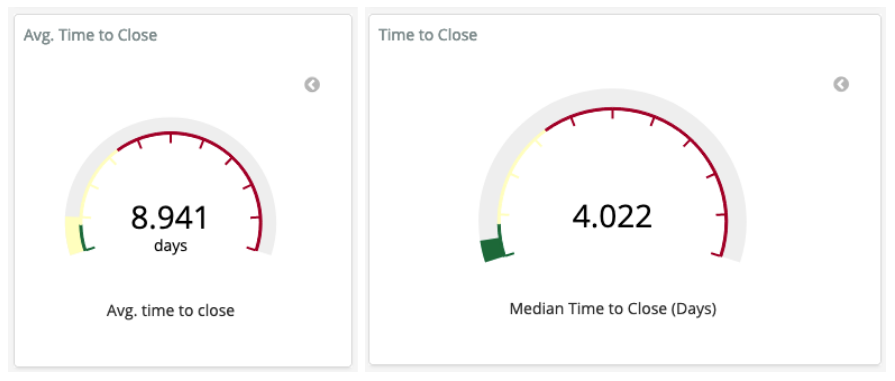
\includegraphics{images/time-to-close_1.png}

\hypertarget{tools-providing-the-metric}{%
\subsubsection{Tools Providing the
Metric}\label{tools-providing-the-metric}}

Augur implementation:

\begin{itemize}
\tightlist
\item
  \href{http://augur.osshealth.io/api_docs/\#api-Evolution-Closed_Issue_Resolution_Duration(Repo)}{Issue
  Close Duration}\\
\item
  \href{http://augur.osshealth.io/api_docs/\#api-Evolution-issue-duration-repo}{Issue
  Duration}\\
\item
  \href{http://augur.osshealth.io/api_docs/\#api-Evolution-Issue_Response_Time(Repo)}{Issue
  Response Time}
\end{itemize}

GrimoireLab implementation:

\begin{itemize}
\tightlist
\item
  \href{https://chaoss.github.io/grimoirelab-sigils/panels/github-pullrequests-efficiency/}{Pull
  Requests Efficiency}\\
\item
  \href{https://chaoss.github.io/grimoirelab-sigils/panels/github-issues-efficiency/}{Issues
  Efficiency}\\
\item
  \href{https://chaoss.github.io/grimoirelab-sigils/panels/efficiency-timing-overview/}{Efficiency:TimingOverview}
\end{itemize}

\hypertarget{data-collection-strategies}{%
\subsubsection{Data Collection
Strategies}\label{data-collection-strategies}}

The time to close metric may be contextual based on the project activity
and objectives. For example, the time to close a bug report may provide
different information than the time to close a new feature request. Data
collection strategies should address different project objectives. Other
variables that may influence these processes are:

\begin{itemize}
\tightlist
\item
  Issue Tracking Systems: the type of issue such as bug report,
  blueprint (OpenStack nomenclature), user story, feature request, epic,
  and others may influence how long this event takes to be closed. Other
  variables, such as the priority or severity may help to advance how
  quickly this event will be closed.\\
\item
  Change Request Processes: this depends on the change request
  infrastructure, as Gerrit, GitHub or mailing lists (as in the Linux
  Kernel) and may differ depending on how complicated the process is.
  For example, newcomers or advanced and experienced developers will
  proceed in different ways and with more or less time required.\\
\item
  Question and Answer Forum: this depends on the quality of the answer
  and the opinion of the person asking the question. A valid answer is
  marked, and the process is closed once the person questioning has
  successfully found a correct answer to their question.
\end{itemize}

\hypertarget{references}{%
\subsection{References}\label{references}}

\begin{itemize}
\tightlist
\item
  ``Practice P.12: Respond to all submissions'' from ``Appendix to:
  Managing Episodic Volunteers in Free/Libre/Open Source Software
  Communities'' by Ann Barcomb, Klaas-Jan Stol, Brian Fitzgerald and
  Dirk Riehle:
  \url{https://opus4.kobv.de/opus4-fau/frontdoor/index/index/docId/13519}
\end{itemize}
 
\hypertarget{time-to-first-response}{%
\section{Time to First Response}\label{time-to-first-response}}

Question: How much time passes between when an activity requiring
attention is created and the first response?

\hypertarget{description}{%
\subsection{Description}\label{description}}

The first response to an activity can sometimes be the most important
response. The first response shows that a community is active and
engages in conversations. A long time to respond to an activity can be a
sign that a community is not responsive. A short time to respond to an
activity can help to engage more members into further discussions and
within the community.

\hypertarget{objectives}{%
\subsection{Objectives}\label{objectives}}

Identify cadence of first response across a variety of activities,
including PRs, Issues, emails, IRC posts, etc. Time to first response is
an important consideration for new and long-time contributors to a
project along with overall project health.

\hypertarget{implementation}{%
\subsection{Implementation}\label{implementation}}

Time to first response of an activity = time first response was posted
to the activity - time the activity was created.

\hypertarget{filters}{%
\subsubsection{Filters}\label{filters}}

\begin{itemize}
\tightlist
\item
  Role of responder, e.g., only count maintainer responses
\item
  Automated responses, e.g., only count replies from real people by
  filtering bots and other automated replies
\item
  Type of Activity, e.g., issues (see metric
  \href{https://github.com/chaoss/wg-evolution/blob/master/metrics/Issue_Response_Time.md}{Issue
  Response Time}), emails, chat, change requests
\end{itemize}

\hypertarget{visualizations}{%
\subsubsection{Visualizations}\label{visualizations}}

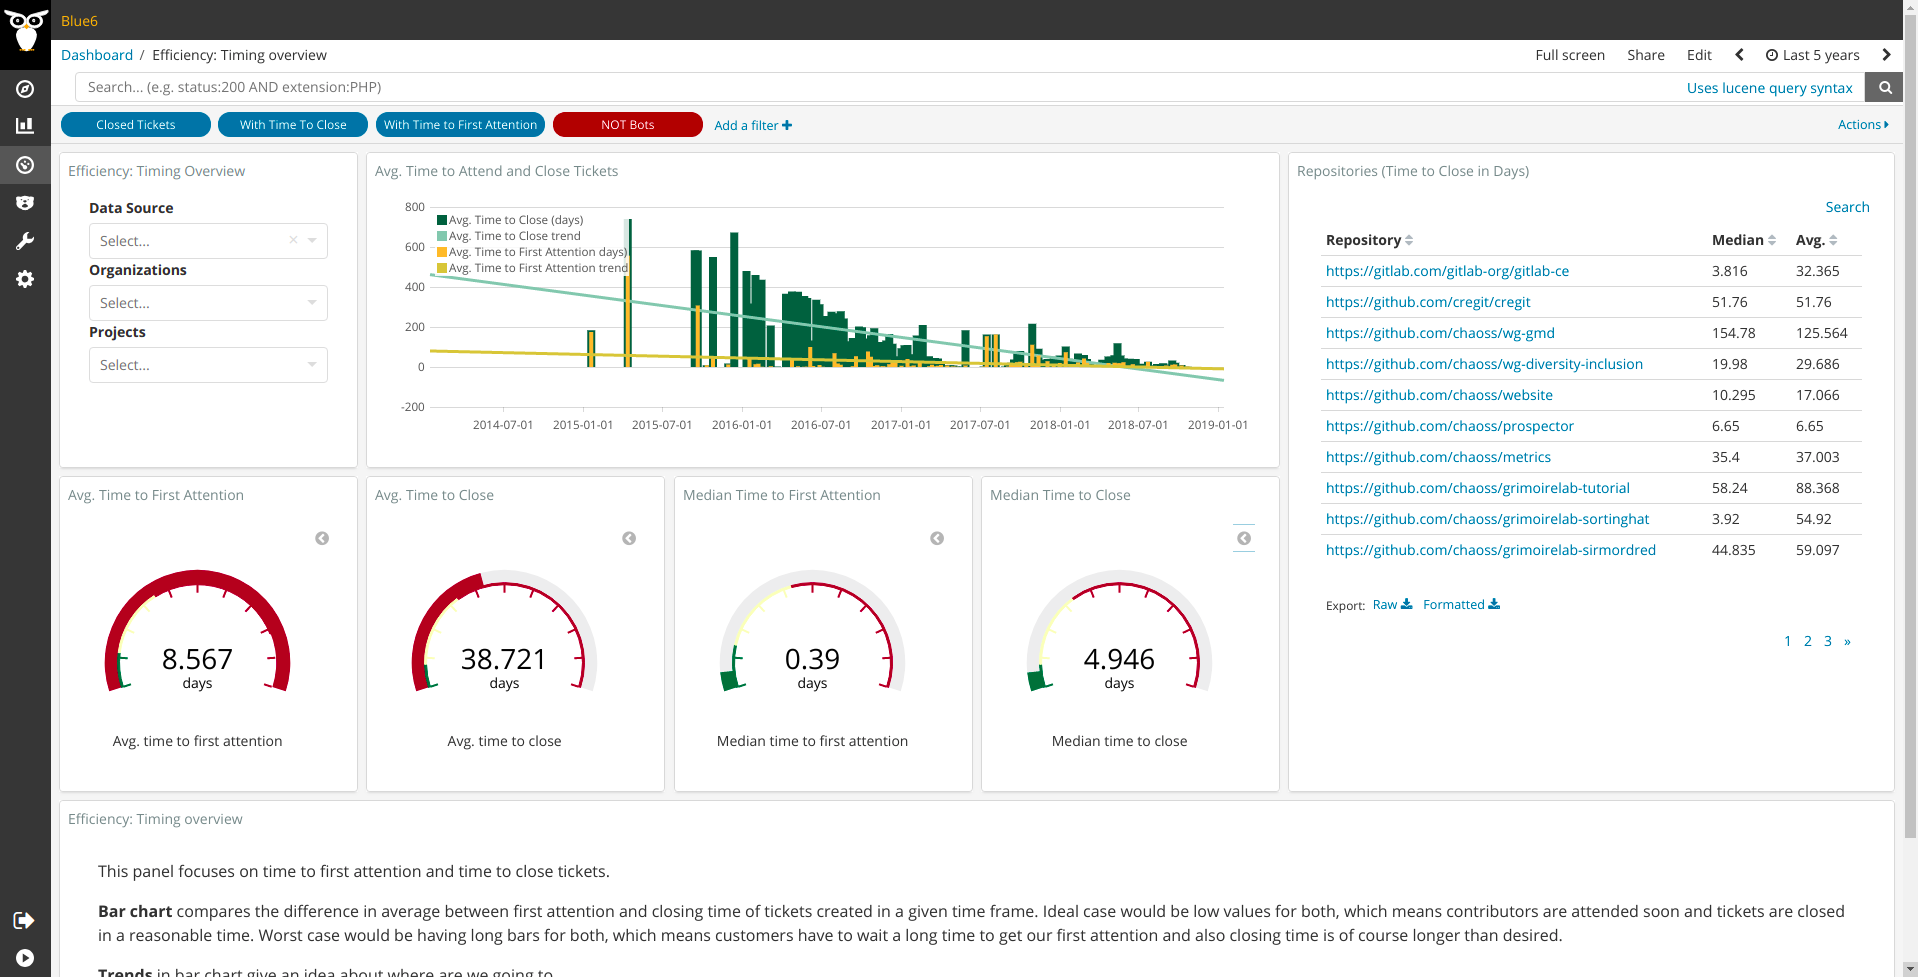
\includegraphics{images/time-to-first-response_efficiency-timing-overview.png}

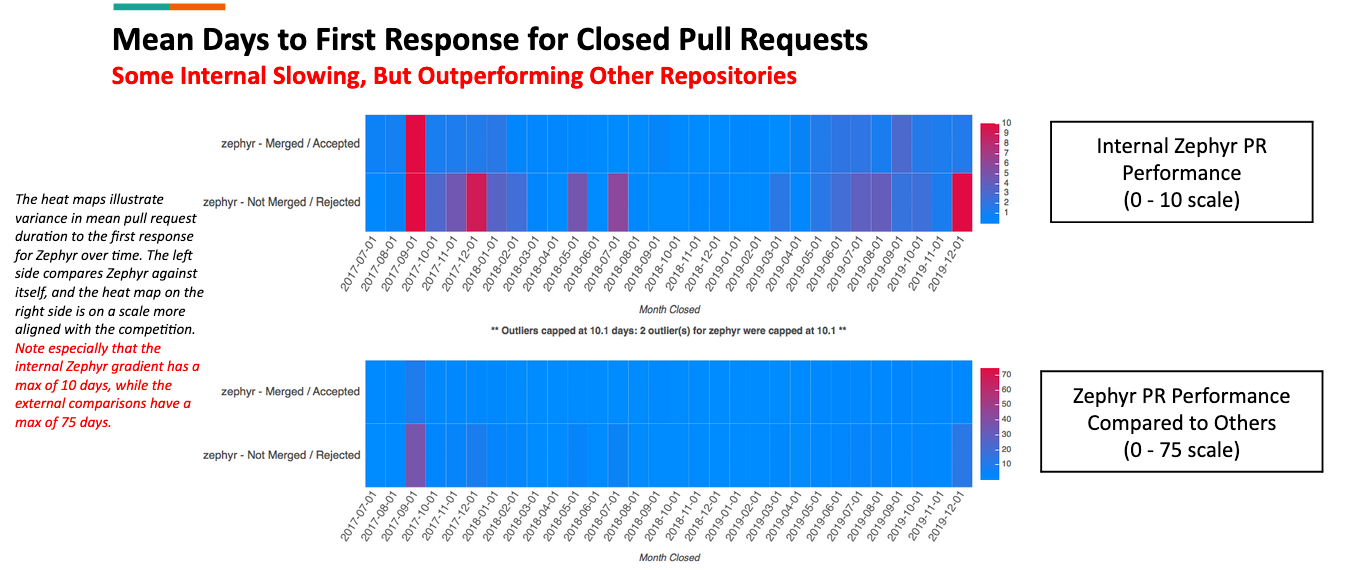
\includegraphics{images/time-to-first-response_augur-ttc-1.png}

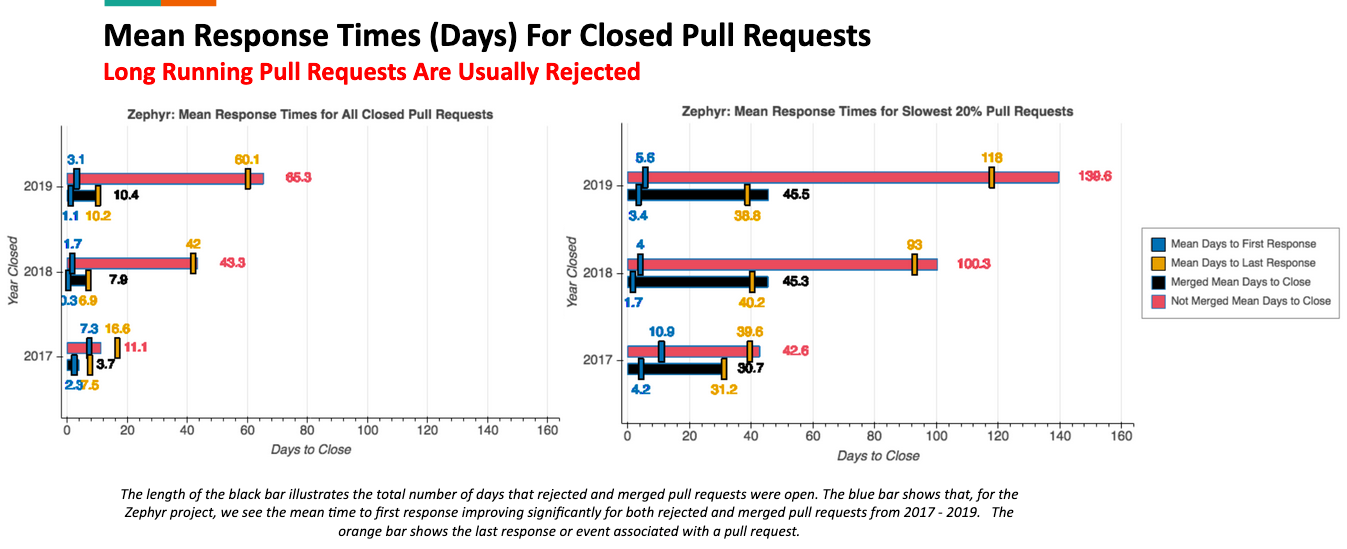
\includegraphics{images/time-to-first-response_augur-ttc-2.png}

\hypertarget{tools-providing-the-metric}{%
\subsubsection{Tools Providing the
Metric}\label{tools-providing-the-metric}}

\begin{itemize}
\tightlist
\item
  GrimoireLab Panel:
  \href{https://chaoss.github.io/grimoirelab-sigils/panels/efficiency-timing-overview/}{Efficiency
  Timing Overview}
\item
  \href{https://katacontainers.biterg.io/app/kibana\#/dashboard/cbbdd920-288c-11e9-b662-975152e57997}{Kata
  Containers dashboard efficiency panel}
\end{itemize}

\hypertarget{references}{%
\subsection{References}\label{references}}
 
